\documentclass{article}

\usepackage[utf8]{inputenc}
\usepackage{polski}
\usepackage[utf8]{inputenc}
\usepackage{listings}
\usepackage{caption}
\usepackage{color}
\usepackage{graphicx}
\usepackage{listings}
\usepackage{hyperref}


\definecolor{dkgreen}{rgb}{0,0.6,0}
\definecolor{gray}{rgb}{0.5,0.5,0.5}
\definecolor{mauve}{rgb}{0.58,0,0.82}

\lstset{frame=tb,
  language=Python,
  aboveskip=3mm,
  belowskip=3mm,
  showstringspaces=false,
  columns=flexible,
  basicstyle={\small\ttfamily},
  numbers=none,
  captionpos=t,
  numberstyle=\tiny\color{gray},
  keywordstyle=\color{blue},
  commentstyle=\color{dkgreen},
  stringstyle=\color{mauve},
  breaklines=true,
  breakatwhitespace=true,
  tabsize=3
}

\DeclareCaptionFormat{listing}{#1#2#3}
\captionsetup[lstlisting]{format=listing,singlelinecheck=false, margin=0pt}



\title{Factorer MPI - dokumentacja projektowa}

\date{2016-06-07}

\author{Rafał Duraj, Piotr Dowgiałło, Bartosz Janusz, Maciej Kolański}

\begin{document}

%generowanie strony tytułowej
\pagenumbering{gobble}
\maketitle
\newpage  
\pagenumbering{arabic}

%spis treści
\tableofcontents
\newpage

\section{Temat projektu}

\paragraph{}W dzisiejszych czasach, gdy właściwie wszystko co robimy w jakiś sposób połączone jest z Internetem bezpieczeństwo jest bardzo ważnym tematem.

Faktoryzacja jest to proces podczas którego dla zadanego obiektu odnajduje się inne obiekty, które spełniają to, że ich iloczyn równy jest oryginalnemu obiektowi, w związku z czym te znalezione czynniki są w pewnym sensie od niego prostsze.

Podstawowy algorytm faktoryzacji bazuje na próbowaniu podziału liczby do faktoryzacji n przez wszystkie liczby pierwsze od 2 do $\sqrt{n}$. Tego typu algorytm bardzo dobrze radzi sobie z początkiem faktoryzacji liczby, bo dowolna liczba ma czynnik zarówno małe jak i duże. Jak wiadomo połowa wszystkich liczb dzieli się przez dwa, jedna trzecia licz przez trzy i tak dalej, a więc z dużym prawdopodobieństwem można pozbyć się w prosty sposób niskich czynników.

RSA jest to jeden z pierwszych i też obecnie najpopularniejszych asymetrycznych algorytmów kryptograficznych gdzie klucz jest publiczny. Bezpieczeństwo szyfrowania przy pomocy tego algorytmu jest związane z trudnością faktoryzacji dużych liczb.

\section{Zakres projektu}
\subsection{Cel}

\paragraph{}Celem projektu jest umożliwienie zlecenia zadania faktoryzacji dużej liczby (większych od $2^{64} -1$). Jednym z głównych założeń jest udostępnienie prostego w obsłudze interfejsu użytkownika i zmaksymalizowanie elastyczności – system powinień być zdolny do współpracy z zadanymi komputerami, a instalacja wymaganego oprogramowania musi być prosta. 

\subsection{Funkcjonalność}

\paragraph{Podstawowa}
\begin{enumerate}
	\item Udostępnienie mechanizmów rejestracji i logowania (konta użytkowników)
	\item Zarządzanie zadaniami z poziomu interfejsu webowego
	\begin{enumerate}
		\item zlecanie zadań
		\item przegląd historii
	\end{enumerate}
	\item Możliwość rozbudowy klastra bez ingerencji w kod
	\item Faktoryzacja metodą „brutalnej siły”
	\item Faktoryzacja metodą CFRAC
	\item Zachowywanie wyników pomyślanie wykonanych faktoryzacji
\end{enumerate}

\paragraph{Rozszerzona}
\begin{enumerate}
    \item Łamanie szyfru RSA
    \item Faktoryzacja metodą sita kwadratowego
    \item Forma graficznej prezentacji wyników pomiarów
\end{enumerate}

\section{Narzędzia i technologie zastosowane w projekcie}
\subsection{Zastosowane technologie}

\begin{figure}[h]
    \centering
    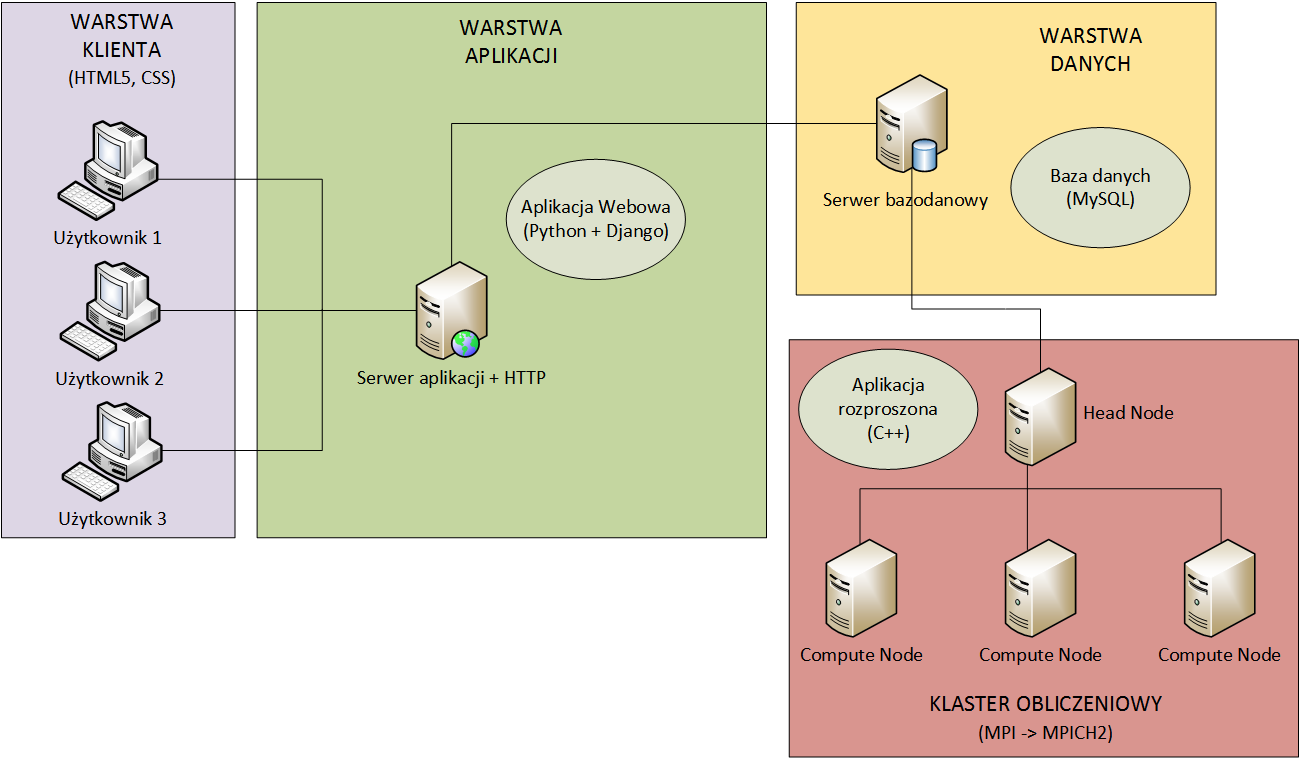
\includegraphics[width=1.0\textwidth]{schemat_blokowy_systemu.png}
    \caption{Schemat blokowy systemu}
    \label{fig:schemat}
\end{figure}

\paragraph{Strona klienta - HTML5, CSS}
Interfejs z którego bedzie korzystal klient projektowanego systemu został napisany w jezyku skryptowym HTML5 z użyciem stylów CSS. HTML5 jest obecnie standardem przy tworzeniu stron internetowych i w wiekszosci wyparl HTML4, w którego specyfikacji bylo duzo niescislosci. Uzycie CSS z kolei pozwoli ujednolicic prezentacje zawartosci w różnych przegladarkach, oraz uprosci organizacje samego kodu.

\paragraph{Aplikacja Webowa - Python 3.4 + Django 1.8.7\cite{django}}
Python jest jezykiem wysokiego poziomu ogólnego przeznaczenia, z kolei Django to framework webowy dla tego jezyka. Wybralismy ten zestaw z powodu wielu ulatwień przy tworzeniu aplikacji webowych, które sa przezeń oferowane, np. dynamiczny interfejs bazy danych, automatyczny interfejst administracyjny. Dodatkowo czesc naszej grupy jest zaznajomiona z tymi technologiami, wiec nie ma potrzeby poznawania ich od zera. Istotne sa tutaj wersje srodowisk - najnowsze dystrybucje nie obsluguja MySQL, w zwiazku z tym wybralismy poprzednie.

\paragraph{Baza danych - MySQL}
SZBD rozwijany przez firme Oracle. Charakteryzuje sie wszystkimi najwazniejszymi funkcjonalnosciami bazy danych oraz prostota tworzenia takiej bazy. Rozważalismy zastosowanie systemu Oracle Database, jednakże jest on zbyt rozbudowany jak na nasze potrzeby, a co za tym idzie trudny w obsudze. Mamy również doswiadczenie w integracji bazy MySQL z aplikacjami napisanymi w Pythonie (Django).

\paragraph{Klaster obliczeniowy - standard MPI\cite{mpich2}} MPICH2 to darmowa implementacja standardu MPI dla systemów Linux. Umożliwa proste tworzenie klastrów obliczeniowych, rozdzielania zadań miedzy poszczególne wezly i zbierania wyników. Oferuje interfejs dla jezyka C++. Jest wykorzystywany w wiekszosci topowych urzadzen wieloprocesorowych i ta popularnosc znaczaco wplynelo na jego wybór.

\paragraph{Aplikacaja rozproszona - C++11}
Wybór padl na ten jezyk ze wzgledu na jego znajomosc przez czlonków grupy oraz interfejs udostepniany przez srodowisko MPICH2.

\subsection{Narzedzia wykorzystane w projekcie}
\begin{itemize}
\item Aplikacja webowa PyCharm 5.0.4 - IDE do Pythona, obsuguje Django
\item Aplikacja rozproszona - CodeLite 9.1 IDE do C++, wersja na system Linux
\item Baza danych - developer do MySQL
\item Organizacja pracy - Trello (\url{https://trello.com/})
\item Hosting plików - GitHub (\url{https://github.com/}) 
\end{itemize}

\section{Aktualny stan rynku\cite{cfracinz}}

\paragraph{GGNFS (GPL'd implementation of General Number Field Sieve)} Aktywny rozwój. faktoryzacja liczb do 180 znaków, srednio do 140. Kilka wiekszych liczb tez. W wiekszosci przypadkow program GGNFS jest stabilny dla liczb skladajacych sie do 150-160 znakow. Posiada bugi. Nie jest czarna skrzynka, trzeba miec odpowiednia wiedze zeby go uzywać.

\paragraph{Cunningham Project} Projekt faktoryzujacy liczby $b^n +-1$ dla b=2,3,5,6,7,10,11,12 i duze n.\cite{cun}

\paragraph{RSA Factoring Challenge} Zawody zorganizowane przez RSA Security. Otwarte zawody dla wszystkich mające na celu zwiększyć zainteresowanie faktoryzacją liczb. Opublikowana została lista pseudopierwszych liczb (rozkładających się na dokładnie dwa czynniki), nazwanych liczbami RSA.Za rozłożenie niektórych z nich wyznaczono pieniężną nagrodę. Najmniejsza z nich, 100-cyfrowa liczba RSA-100 została rozłożona w ciągu kilku dni, ale większość do dziś pozostaje niezłamana.Zawody miały na celu śledzenie rozwoju możliwości komputerów w faktoryzacji. Jest to niezwykle istotne przy wyborze długości klucza w szyfrowaniu asymetrycznym metodą RSA. Postęp w łamaniu kolejnych liczb powinien zdradzać jakie długości klucza można jeszcze uznawać za bezpieczne.\cite{rsafactoringchallenge}

\paragraph{}Poczatkowo rekordy były bite za pomoca algorytmu CFRAC, który ustapił dopiero w latach 8X algorytmowi sita kwadratowego. Za pomoca algorytmu QS sfaktoryzowano, miedzy innymi, liczby $RSA-100, RSA-110, RSA-120 i RSA-129$. Następnie na scene wkroczył algorytm sita ciałliczbowego, który do dzis pozostaje najszybszym ze znanych algorytmów faktoryzacji i dzierży rekordy - najpierw RSA-640 (640 bitów, 193 cyfry) i RSA-200 (200 cyfr) w 2005 roku, a następnie RSA-768(232 cyfry) w 2009 roku, co pozostaje niepobitym rekordem do dzis.

\section{Projekt techniczny}

\subsection{Klaster obliczeniowy - Komunikacja}

\paragraph{}Program realizujący obliczenia został zrealizowany w oparciu o architekturę Master-Slave, a użytkownik systemu może uruchamiać kolejne zadania poprzez komunikację z węzłem Master. W tym celu określony został interface {\it FactorerCommunictorInterface} i jego dwie implementacje, z których jedna służy do komunikacji z klastrem przy użyciu konsoli (uruchomienie programu z parametrem cmd), a druga z bazą danych (stroną internetową). Metoda {\it getCommand} pobiera polecenie (od użytkównika lub bazy danych), a {\it algorithmFinished} przesyła wynik obliczeń. Takie podejście pozwala na abstrakcyjne podejście do tematu komunikacji - algorytm nie jest powiązany z bazą lub stroną internetową i z łatwością można dodać implementację pobierającą danę z innego źródła. 

\begin{lstlisting}[caption=Interface wykorzystany do komunikacji]
enum CommunicatorCommand{Quit, Algorithm};

class FactorerCommunicatorInterface
{
public:
    virtual ~FactorerCommunicatorInterface() {};

    virtual CommunicatorCommand getCommand(MPIAlgorithm::AlgorithmsEnum &algorithm, std::string &number ) = 0;
    virtual void algorithmFinished(const std::vector<std::string> &result) = 0;

    static std::string commandAsString(CommunicatorCommand command) 
\end{lstlisting}

\paragraph{}Najważniejszym dla projektu sposobem komunikacji jest implementacje łącząca klaster z bazą danych - to ona umożliwia zlecanie zadań z poziomu strony internetowej. W trakcie realizacji projektu rozważano także podejście wykorzystujące bezpośrednie połączenie pomiędzy serwerem strony, a węzłem master, zdecydowano się jednak na wykorzystanie pośredniczącej bazy danych z następujących przyczyn:
\begin{itemize}
\item Użycie Django właściwie wymaga wykorzystania bazy danych do przechowywania danych, więc element musiał pojawić się w projekcie.
\item Jednocześnie Django zapewnia bardzo dobre wsparcie w komunikacji z bazą danych.
\item Podejście tego typu zapewnia modularność - do systemu można dodać klienta innego typu niż strona WWW (np. aplikację mobilną) z zerowym kosztem, dane byłby przesyłane do bazy dokładnie w ten sam sposób, sam klaster nie musi znać ich źródła.
\item Liczba klastrów także staje się nieograniczony, każdy może pobierać wolne zadanie z bazy danych w dowolnej chwili.
\end{itemize}

\subsection{Klaster obliczeniowy - Algorytm Brute Force}

\subsection{Klaster obliczeniowy - Algorytm CFRAC}
\subsubsection{Opis algorytmu\cite{cfracwiki}\cite{cfracinz}}
\paragraph{}Metoda CFRAC  jest algorytmem faktoryzacji liczb całkowitych. Jest to uniwersalny algorytm będący w stanie rozłożyć na czynniki każdą liczbę, nie polegając na żadnych ograniczeniach czy warunkach. Został on opisany przez D.H. Lehmer'a oraz R. E. Powers'a w 1931 roku, oraz wdrożony na komputery pierwszy raz przez Michael'a A. Morisson'a oraz John'a Brillhart'a w 1975 roku.

\paragraph{}Algorytm ten bazuje na metodzie faktoryzacji Diaxona. Metoda Diaxona polegała na losowaniu kolejnych liczb 'a' takie, że:
$sqrt[n] < a < n$ (gdzie n to liczba, którą chcemy sfaktoryzować)
i sprawdzamy(używając algorytmu naiwnego), czy $b^2 = a^2mod(n)$ jest liczbą B-gładką, dla ustalonego B. Jeżeli tak to dodajemy znalezioną parę do zbioru (liczba B-gładka to taka liczba, której wszystkie dzielniki pierwsze są mniejsze bądź równe dla ustalonego B).

\paragraph{}W algorytmie CFRAC idea pozostaje bez zmian, definiowany jest natomiast sposób wybierania par. Zamiast losowania ich wykorzystywany jest ciąg rozwinięcia sqrt(n) w ułamek łańcuchowy. Złożoność obliczeniowa algorytmu CFRAC jest rzędu $O(e^sqrt(2* logn * loglog n))$ <- na wikipedi lepiej przedstawiony wzor

\subsubsection{Implementacja\cite{cfracimpl}}
\paragraph{}Program generuję rekurencyjnie elementy tablicy, której elementy są ze sobą ściśle powiązane, następującymi wzorami:

$Q[n] = Q[n-2] + q[n-1] * (r[n-1] - r[n-2]) G[n] = 2g - r[n-1] q[n] = G[n]/Q[n] r[n] = G[n] - q[n]Q[n] A[n] = q[n]*A[n-1] + A[n-2]modN$

gdzie

$Q[-1]= N Q[0] = 1 q[0] = g r[-1] = g r[0] = 0 A[-1]= 1 A[0] = g g = sqrt(N)$
\paragraph{}Dla powyższych reguł generowane są rekurencyjnie kolejne rekordy. Przy wygenerowaniu każdego kolejnego "zestawu" wyników badany był element Q[i]. Jeżeli był on możliwy do spierwiastkowania(reszta z pierwiastka kwadratowego jego wartości była równa zeru), to następnym krokiem w celu uzyskania szukanego faktora było obliczenie następującej wartości:

$temp = A[i-1] - sqrt(Q[i])$

\paragraph{}Ostatnim krokiem było obliczenie NWD (największego wspólnego dzielnika)pomiędzy uzyskaną wartością (temp), a liczbą dla której szukamy faktora(N). Wykorzystanym algorytmem do obliczania NWD był algorytm euklidesa, który jest aktualnie najefektywniejszym algorytmem wykorzystywanym do tej operacji.

\subsubsection{Podział zadań (Master Slave)}

\paragraph{}Z powodu rekurencyjnego generowania wyników, efektywny podział pracy pomiędzy różne maszyny(slave'y) był bardzo ciężki do zrealizowania. Ostatecznie udało nam się wymyślić sposób podziału prac, który może nie jest najlepszy ale zapewnia w pewnym stopniu poprawe wydajności przy wykorzystaniu wielu maszyn.

\paragraph{}Polega on na wprowadzeniu do algorytmu parametru K. Dla każdej maszyny oprócz danej liczby do faktoryzacji wysyłamy również indywidualny dla niej parametr, przez który mnoży on otrzymaną liczbę do faktoryzacji. Dla nowej uzyskanej liczby k*N, algorytm znajduję wyniki w innym czasie. Wadą tego rozwiązania jest nie zawsze poprawny wynik, dlatego po jego odebraniu trzeba sprawdzić jego poprawność (np odrzucić wyniki, które dzielą się przez k)

\paragraph{}Należy też wspomnieć, że CFRAC jest efektywnym algorytmem tylko dla dużych liczb, dlatego w celu znacznego skrócenia czasu operacji mniejsze liczby faktoryzowane są prostym algorytmem naiwnym przez maszyne Master.

\paragraph{}Algorytm podziału zadań przez maszyna Master wygląda w następujący sposób:

\begin{lstlisting}[caption=Sekwencja instrukcji algorytmu CFRAC,numbers=left]
    Utworz kolejke na wynik
    Wrzuc pierwsza liczbe (N) do kolejki liczb do faktoryzacji
    Dopoki kolejka nie jest pusta 
        Dopoki nie znalazles ostatniej liczby pierwszej
            Wyciagnij liczbe A z kolejki 
            Jezeli A jest liczba duza //(efektywny CFRAC) 
                Zainicjuj maszyny (Slaves) 
                Rozeslij zadania wraz z indywidualnym parametrem K 
                Wyrzuc aktualna liczbe A z kolejki 
                Wykonuj dopoki nie odbierzesz wynikow od wszystkich maszyn 
                    Czekaj na wynik 
                    Sprawdz jego poprawnosc 
                    Jezeli wynik jest poprawny: 
                        Jezeli jest liczba pierwsza, wrzuc do kolejki wynikow
                        Jezeli nie jest liczba pierwsza wrzuc go oraz jego iloraz z liczba A do kolejki liczb do faktoryzacji 
                    Jezeli zadna maszyna nie zwrocila poprawnego wyniku, zmien parametr k i wrzuc z powrotem liczbe A do kolejki liczb do faktoryzacji 
            Dla malej liczby uzyj algorytmu naiwnego (bruteforce)
\end{lstlisting}

\subsection{Strona internetowa}

Dostępna w sieci Internet strona WWW finalnie umożliwia rejestrację i logowanie użytkowników oraz zlecanie zadań, czyli liczb do faktoryzacji. Do tego użytkownik ma wgląd w historię zleconych przez niego zadań wraz z ich rozwiązaniami. Poza funkcjonalnościami dla zwykłego użytkownika strona umożliwia także działania administracyjne poprzez panel administracyjny. Do zadań tych należą takie rzeczy jak usuwanie zleconych zadań, nadawanie im priorytetu czy też zarządzanie użytkownikami. Strona współpracuje z bazą danych MySQL. Jest ona dostępna pod adresem \url{http://156.17.235.48/}.

\newpage
\begin{figure}[h!]
    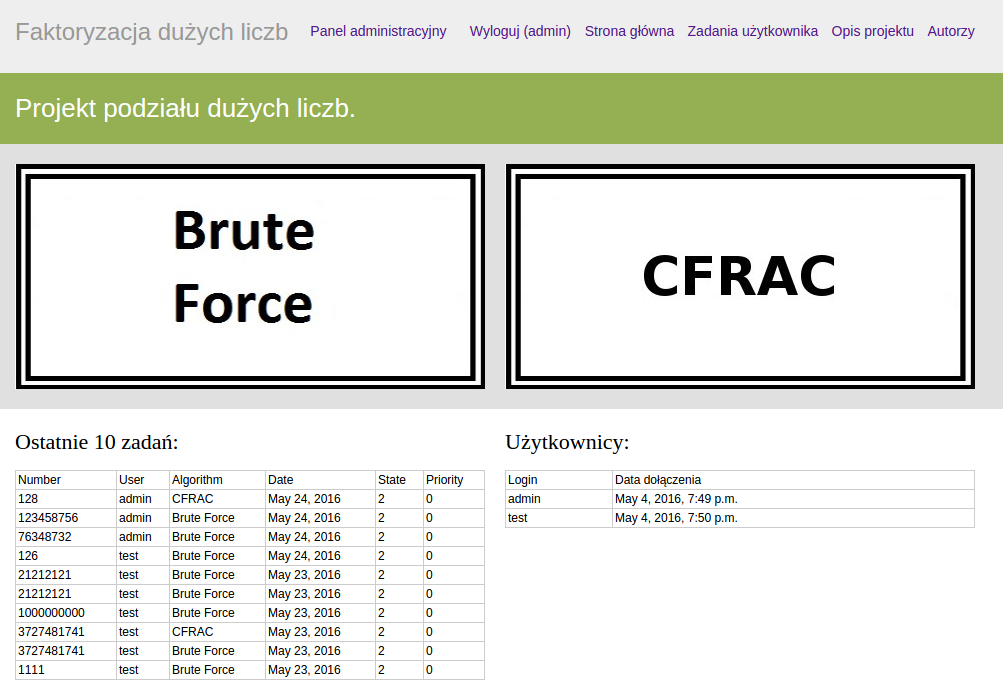
\includegraphics[width=\linewidth]{mainpage.png}
    \caption{Strona główna.}
    \label{fig:mainpagescr}
\end{figure}

Stronę wykonano przy użyciu technologii Python Django\cite{django} i edytora tekstowego Sublime\cite{sublime} wraz z dodatkiem Anaconda Python IDE\cite{anacondaide}. Do komunikacji z bazą danych wykorzystano standardową bibliotekę do połączenia z MySQL dostępną w Django. Baza danych została stworzona przy pomocy ORM\cite{orminfo} także standardowego dla Django. Przykładowy kod dla encji Task poniżej.

\begin{lstlisting}
class Task(models.Model):
    CANCELLED_STATUS = -1
    UNDONE_STATUS = 0
    WORKING_STATUS = 1
    DONE_STATUS = 2
    STATUS_CHOICES = (
        (CANCELLED_STATUS, "Cancelled"),
        (UNDONE_STATUS, "Undone"),
        (WORKING_STATUS, "Working"),
        (DONE_STATUS, "Done")
    )

    number_to_factor = models.CharField(max_length=200)
    job_date = models.DateField(default=timezone.now)
    state = models.IntegerField(choices=STATUS_CHOICES, default=UNDONE_STATUS)
    priority = models.IntegerField(default=0)
    result = models.CharField(max_length=200)
    user = models.ForeignKey(User, on_delete=models.CASCADE)
    algorithm = models.ForeignKey(Algorithm, on_delete=models.CASCADE)

    def __str__(self):
        return str(self.number_to_factor)
\end{lstlisting}

Kolejne kolumny danej tabeli w bazie danych są tworzone poprzez definiowanie pól klas dziedziczących po models.Model\cite{djangomodels}, tak jak powyżej na przykład kolumna result jest polem tekstowym o długości maksymalnej 200 znaków. \\

W celu utworzenia nowej podstrony definiuje się klasy dziedziczące po klasie View z Django. Poniżej znajduje się kod dla widoku podstrony z zadaniami użytkownika.

\begin{lstlisting}
class UserView(LoggedInMixin, View):
    template_name = 'FactorerMain/userview.html'

    def get(self, request, *args, **kwargs):
        tasks = Task.objects.filter(user=request.user.id)[::-1]

        context = {'tasks': tasks}

        return render(request, self.template_name, context)
\end{lstlisting}

W tym przypadku UserView dziedziczy również po klasie LoggedInMixin odpowiadającej za autoryzację, dzięki czemu do takiej podstrony ma dostęp tylko użytkownik zalogowany. W zmiennej template\_name wskazano na szablon strony opisany w języku HTML. Następnie w metodzie get pobierane są wyniki z bazy danych przy pomocy metody Task.objects.filter(user=request.user.id)[::-1]. Zwróci to z encji Task wyniki należące do aktualnego użytkownika posortowane w od najnowszych do najstarszych. Na końcu zwracany jest szablon oraz kontekst, w tym przypadku zadania użytkownika, poprzez metodę render.\\

Można tak pobrane dane z bazy użyć w HTML i wyświetlić je na stronie. Kod wygląda następująco:

\begin{lstlisting}
<h2>Moje zadania:</h2>

    
        <details>
        <summary><p>Liczba <b>{{ task.number_to_factor }}</b> przy uzyciu {{ task.algorithm }} dnia {{ task.job_date }} jest w stanie {{ task.state }}</p></summary>
                 
            {{ task.result }}
        </p>
        
        </details>
    </br></br>  
      

    <p>No tasks to show.</p>

\end{lstlisting}

Pierw sprawdzane jest czy w kontekście została przekazana zmienna tasks. Następnie przy pomocy pętli for przechodzi się przez kolejne elementy tabeli i drukuje jej elementy przy pomocy składni [tabela].[element]. Przykład uzyskanych z bazy danych wyników na stronie pokazano na rysunku poniżej.

\begin{figure}[h!]
    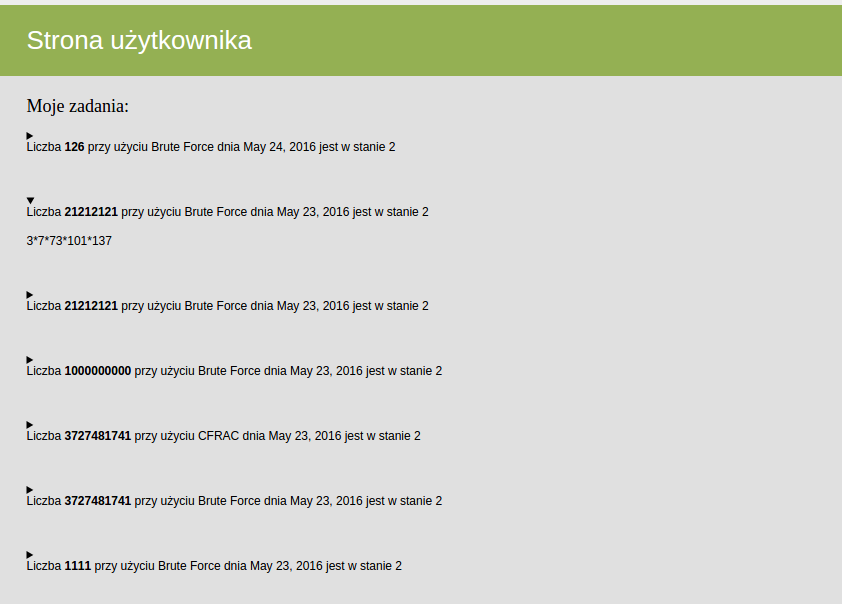
\includegraphics[width=\linewidth]{userpage.png}
    \caption{Podstrona z zadaniami użytkownika.}
    \label{fig:userpagescr}
\end{figure}

W Django zazwyczaj definiuje się jeden bazowy szablon w postaci pliku HTML, a następnie na podstronach zastępuje się tylko wyróżnione bloki strony w sposób wyspecyfikowany dla danej podstrony. Uzyskuje się to przez rozszerzanie szablonów. Dla przykładu w główny pliku HTML znajduje się następujący fragment:

\begin{lstlisting}
 <div id="portfolio-samples">
    <div class="wrap clearfix">
        
        
    </div><!-- // end .wrap -->
</div><!-- // end #portfolio-samples -->
\end{lstlisting}

W tym kodzie zdefiniowano blok gallery, można go zastąpić przy pomocy poniższego fragmentu na innej stronie. 

\begin{lstlisting}



<div class="portfolio-item fl col-2">
  <a href=><img src="static/images/al1.jpg" alt="thumb" /></a>
      <div class="info">Brute force</div>
  </div><!-- // end .portfolio-item -->
  <div class="portfolio-item fl push-2 col-2">
      <a href=><img src="static/images/al2.jpg" alt="thumb" /></a>
      <div class="info">CFRAC</div>
  </div><!-- // end .portfolio-item -->

\end{lstlisting}

Poza blokiem gallery reszta strony będzie taka jak zdefiniowano w pliku base.html. Strona projektu składa się z jednego bazowego szablonu i rozszerzających go kilku podstron.\\

W celu połączenia wszystkiego należy zdefiniować jeszcze w pliku urls.py odwzorowania adresów url dla odpowiednich stron, dzięki czemu Django uruchamia odpowiednie klasy widoków dla zadanego adresu.

\begin{lstlisting}
urlpatterns = [
    url(r'^$', views.IndexView.as_view(), name='index'),
    url(r'^userview/?$', views.UserView.as_view(), name='userview'),
    url(r'^about/?$', views.AboutView.as_view(), name='about'),
    url(r'^creators/?$', views.CreatorsView.as_view(), name='creators'),
    url(r'^bruteforce/?$', views.BruteforceView.as_view(), name='bruteforce'),
    url(r'^cfrac/?$', views.CFRACView.as_view(), name='cfrac'),
    url(r'^login/?$', 'django.contrib.auth.views.login'),
    url(r'^logout/?$', 'django.contrib.auth.views.logout'),
    url(r'^register/?$', views.register, name='register'),
    url(r'^success_register/?$', views.SuccessRegisterView.as_view(),
        name='success_register'),
    url(r'^admin/?', include(admin.site.urls)),
]
\end{lstlisting}

Przy tak zdefiniowanych adresach odnosi się do nich w HTML poprzez następującą linię kodu:
\begin{lstlisting}
<a href="">Strona glowna</a>}
\end{lstlisting}

Do zadań administracyjnych został wykorzystany standardowy panel Django administration skonfigurowany dla potrzeb projektu.

\begin{figure}[h!]
    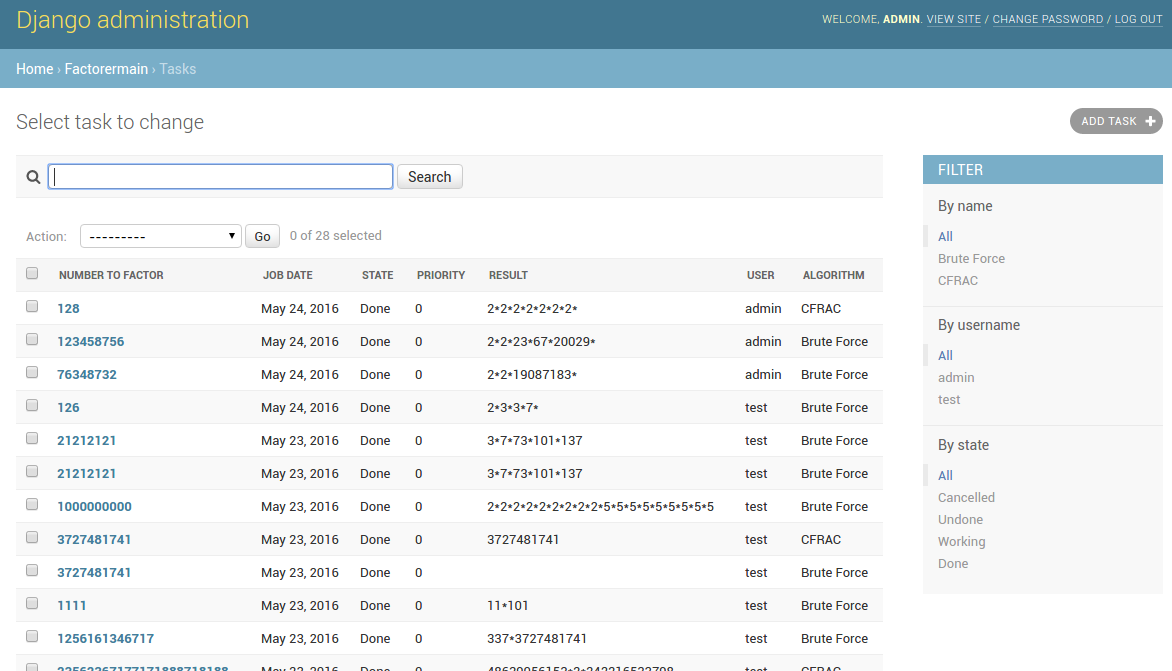
\includegraphics[width=\linewidth]{adminpage.png}
    \caption{Panel administracyjny Django.}
    \label{fig:adminpagescr}
\end{figure}

Panel modyfikuje się poprzez edycję pliku admin.py.

\begin{lstlisting}
class TaskAdmin(admin.ModelAdmin):
    list_display = ('number_to_factor', 'job_date', 'state', 'priority', 'result', 'user', 'algorithm')
    search_fields = ['user__username']
    list_filter = ('algorithm__name', 'user__username', 'state')

admin.site.register(Task, TaskAdmin)
\end{lstlisting}

Klasa musi dziedziczyć po klasie admin.ModelAdmin, następnie można zdefiniować sposób wyświetlania danych, pola, po których ma być realizowane wyszukiwanie, czy też listę filtrów. Na końcu trzeba zarejestrować taką klasę dla danej encji.

\section{Dokumentacja powykonawcza (instalacyjna)}

\subsection{Uruchomienie klastra}
\subsubsection{Wymagania systemowe}

System posiada następujące wymagania programowe:
\begin{itemize}
\item system operacyjny Ubuntu 14.04 LTS
\item zainstalowana biblioteka MPICH2 w wersji 3.0.4
\item klient SSH, np. openssh (1:6.6p1-2ubuntu2.7)
\item serwer systemu wymiany plików NFS, np. nfs-kernel-server (1:1.2.8-6ubuntu1.2) - na głównej maszynie klastra (master)
\item klient systemu wymiany plików NFS, np. nfs-common (1:1.2.8-6ubuntu1.2) - na pozostałych maszynach klastra (slaves)
\end{itemize}
 
Minimalne wymagania sprzętowe nie zostały sprecyzowane, system powinien się uruchomić na dowolnej konfiguracji z zainstalowanym powyższym oprogramowaniem. Niezbędne jest, aby wszystkie maszyny tworzące klaster były umieszczone w jednej sieci LAN pracującej w technologii FastEthernet lub wyższej. Dodatkowo węzeł główny musi posiadać połączenie z Internetem w celu komunikacji z bazą danych.

\subsubsection{Konfiguracja systemu}
Aby uruchomić system na docelowej grupie maszyn należy wykonać następujące kroki:
\begin{itemize}
\item zmapować adresy ip maszyn w pliku systemowym \textit{/etc/hosts}
\item utworzyć na każdej maszynie nowego użytkownika \textit{mpiuser}
\item utworzyć folder współdzielony w sieci za pomocą systemu NFS
\item zapewnić bezhasłowe połączenie SSH pomiędzy węzłem głównym, a każdym węzłem obliczeniowym
\item skopiować plik wykonywalny programu do folderu współdzielonego
\item uruchomić plik za pomocą komendy \textit{mpirun}
\end{itemize}
\newpage
\paragraph{Edycja pliku \textit{hosts}}

Plik znajduje się w katalogu /etc. Należy edytować go w dowolnym edytorze tekstu i przypisać lokalne adresy ip do nazw hostów. Przykładowy plik:
\begin{lstlisting}
127.0.0.1	localhost
#127.0.1.1	linux0

156.17.41.15	master
156.17.41.60	slave1
156.17.41.61	slave2
156.17.41.62	slave3

# The following lines are desirable for IPv6 capable hosts
::1     ip6-localhost ip6-loopback
fe00::0 ip6-localnet
ff00::0 ip6-mcastprefix
ff02::1 ip6-allnodes
ff02::2 ip6-allrouters
\end{lstlisting}

\paragraph{Tworzenie nowego użytkownika}

Aby utworzyć nowego użytkownika należy wykonać następującą komendę z uprawnieniami administratora:
\begin{lstlisting}
$ sudo adduser mpiuser
\end{lstlisting}

Krok należy powtórzyć na każdym węźle.

\paragraph{Utworzenie folderu współdzielonego i udostępnienie go w sieci}
Po zalogowaniu na konto \textit{mpiuser} należy dokonać następujących kroków:

Na głównym węźle:

Utworzenie folderu cloud:
\begin{lstlisting}
$ mkdir cloud
\end{lstlisting}

Edycja pliku /etc/exports i umieszczenie w nim wpisu:
\begin{lstlisting}
/home/mpiuser/cloud *(rw,sync,no_root_squash,no_subtree_check)
\end{lstlisting}

Wyeksportowanie zmian:

\begin{lstlisting}
$ exportfs -a
\end{lstlisting}
\newpage
Na węzłach obliczeniowych:

Utworzenie folderu cloud:
\begin{lstlisting}
$ mkdir cloud
\end{lstlisting}

Zamontowanie folderu współdzielonego do lokalnego systemu plików:
\begin{lstlisting}
$ sudo mount -t nfs master:/home/mpiuser/cloud ~/cloud
\end{lstlisting}

Sprawdzenie, czy folder został poprawnie zamontowany:
\begin{lstlisting}
$ df -h
Filesystem                  Size  Used Avail Use% Mounted on
master:/home/mpiuser/cloud  49G   15G   32G  32% /home/mpiuser/cloud
\end{lstlisting}

\paragraph{Tworzenie bezhasłowego połączenia SSH}
Poniższe kroki należy wykonać na każdym węźle.

Generacja pary kluczy - publicznego i prywatnego:
\begin{lstlisting}
$ ssh-keygen -t dsa
\end{lstlisting}

Przesłanie klucza publicznego z węzła głównego na obliczeniowe i na odwrót:
\begin{lstlisting}
$ ssh-copy-id master (na wezlach obliczeniowych)
$ ssh-copy-id slave[i] (na wezle glownym)
$ ssh-copy-id localhost (dodatkowo na kazdej maszynie)
\end{lstlisting}

Wyłączenie konieczności podawania hasła przy logowaniu SSH:
\begin{lstlisting}
$ eval `ssh-agent`
$ ssh-add ~/.ssh/id_dsa
\end{lstlisting}

Należy przetestować połączenie pomiędzy węzłem głównym i każdym z obliczeniowych za pomocą próby zalogowania:
\begin{lstlisting}
$ ssh master (slave[i])
\end{lstlisting}

\paragraph{Uruchomienie pliku wykonywalnego}
Uruchomienie pliku wykonywalnego Factorer dokonuje się za pomocą komendy mpirun z określonymi parametrami. Przykładowe wywołanie:
\begin{lstlisting}
$ mpirun -np 4 -hosts master,slave1 ./Factorer
\end{lstlisting}

Komenda przyjmuje następujące parametry:
\begin{itemize}
\item -np \textit{liczba} - zbiorcza liczba wątków wykonywanych na klastrze. Przykład:
System składa się z 3 jednakowych maszyn obliczeniowych i węzła głównego. Każda stacja posiada 2 rdzenie procesora. W celu równomiernego zrównoważenia obciążenia procesór wartość parametru powinna wynosić 3*2 + 2 = 8 wątków.

\item -hosts \textit{hostname1},\textit{hostname2} ... - nazwy węzłów na których ma zostać uruchomiony program oddzielone przecinkami (bez spacji). Lista musi zawierać węzeł główny (master) oraz może zawierać dowolną liczbę węzłów obliczeniowych (slave).
\end{itemize}

\subsection{Uruchamianie strony}

W celu uruchomienia strony potrzebny jest serwer wraz z zainstalowaną powłoką Python 3.4. Do tego należy zainstalować moduł Django w wersji 1.8.7. Oprócz powyższych należy też mieć serwer bazy danych, w przypadku tego projektu jest to serwer MySQL. Po spełnieniu tych wymagań można przejść do uruchamiania strony.\\

Pierwszym krokiem jest ustawienie w opcjach strony w pliku settings.py danych dostępowych do bazy danych.
\begin{lstlisting}
DATABASES = {
    'default': {
        'ENGINE': 'django.db.backends.mysql',
        'NAME': 'factorDB',
        'USER': 'projekt',
        'PASSWORD': 'projekt',
        'HOST': '156.17.235.48',
        'PORT': '3306',
    }
}
\end{lstlisting}

Następnym krokiem jest wypełnienie bazy danych odpowiednimi strukturami stworzonymi wcześniej w Python używająć rozwiązania typu ORM. Służy do tego skrypt manage.py znajdujacy się w folderze z plikami źródłowymi strony. Należy zrobić migrację bazy danych dla naszej aplikacji(nazwa to FactorerMain). Osiąga sie to przez wywołanie \textbf{python manage.py makemigrations FactorerMain}. Następnie koniecznym jest wykonać utworzone migrację poprzez \textbf{python manage.py migrate}. Dzięki tym dwóm komendom baza danych zostanie wypełniona odpowiednio zdefiniowanymi strukturami. Ostatnim krokiem jest uruchomienie serwera, osiąga się to przez użycie kolejnej komendy skryput manage.py - \textbf{python manage.py runserver}.
\begin{lstlisting}
$ python manage.py runserver
Performing system checks...

System check identified no issues (0 silenced).

June 08, 2016 - 16:24:25
Django version 1.8.7, using settings 'Factorer.settings'
Starting development server at http://127.0.0.1:8000/
Quit the server with CONTROL-C.

\end{lstlisting}

Jak widać na powyższym wyciągu z terminala serwer został uruchominy.

\section{Istotne elementy kodu z komentarzem}

\newpage
\section{Przykładowe wyniki badań efektywności programu równeległego}
\subsection{Algorytm CFRAC}
\begin{figure}[h]
    \centering
    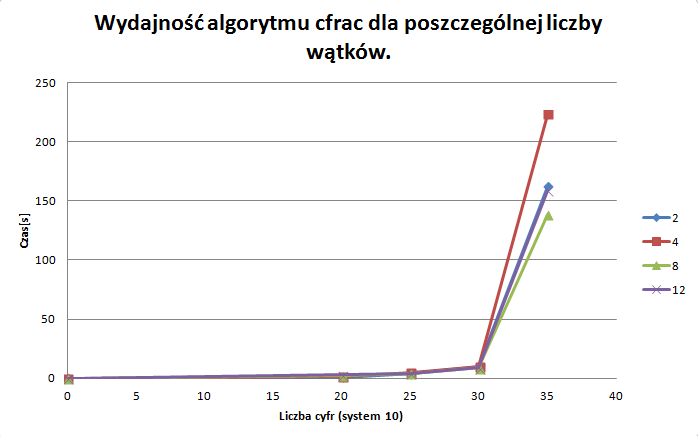
\includegraphics[width=1.0\textwidth]{cfracWydajnosc.png}
    \caption{Wydajność algorytmu CFRAC dla poszczególnej liczby wątków}
    \label{fig:cfracWykres}
\end{figure}
\begin{figure}[h]
    \centering
    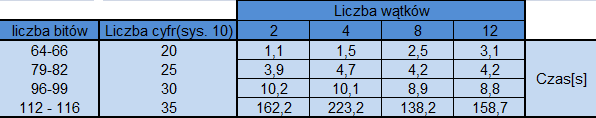
\includegraphics[width=1.0\textwidth]{cfracWydajnoscTabela.png}
    \caption{Dane pomiarów wydajność algorytmu CFRAC}
    \label{fig:cfracTabela}
\end{figure}
\paragraph{}Badania przeprowadzone zostały na pojedyńczym komputerze wykorzystując symulację mpi dla danej ilości wątków.

\section{Wnioski}

\newpage
\begin{thebibliography}{9}
\bibitem{django}
	\emph{Dokumentacja Django}.
	\url{https://docs.djangoproject.com/en/1.8/},
	2016

\bibitem{mpich2}
	\emph{Dokumentacja MPICH2}.
  	\url{http://www.mpich.org/documentation/guides/},
  	2016.

\bibitem{cun}
	\emph{Cunningham Project}.
	\url{http://homes.cerias.purdue.edu/~ssw/cun/}

\bibitem{rsafactoringchallenge}
	\emph{RSA Factoring Challenge}.
	\url{http://pl.wikipedia.org/wiki/RSA_Factoring_Challenge}
	
\bibitem{cfracwiki}
	\emph{CFRAC opis}.
	\url{https://en.wikipedia.org/wiki/Continued_fraction_factorization}

\bibitem{cfracinz}
	\emph{CFRAC zastosowanie}.
	\author{Mateusz Niezabitowski}
    \url{http://ki.agh.edu.pl/sites/default/files/usefiles/172/theses/mateusz.niezabitowski.algorytmy.faktoryzacji.w.zastosowaniach.kryptograficznych.v1.0-final.pdf}
    
\bibitem{cfracimpl}
	\emph{CFRAC implementacja}.
    \url{https://math.dartmouth.edu/~carlp/PDF/implementation.pdf}

\bibitem{sublime}
  \emph{Sublime Text Editor}.
  \url{https://www.sublimetext.com/}

\bibitem{anacondaide}.
  \emph{Anaconda Python IDE}
  \url{http://damnwidget.github.io/anaconda/}

\bibitem{orminfo}
  \emph{ORM - object-relational mapping}.
  \url{https://pl.wikipedia.org/wiki/Mapowanie_obiektowo-relacyjne}

\bibitem{djangomodels}
  \emph{Django Models documentation}.
  \url{https://docs.djangoproject.com/en/1.9/topics/db/models/}

\end{thebibliography}

\end{document}